%%
%% This is file `sample-acmsmall-submission.tex',
%% generated with the docstrip utility.
%%
%% The original source files were:
%%
%% samples.dtx  (with options: `acmsmall-submission')
%%
%% IMPORTANT NOTICE:
%%
%% For the copyright see the source file.
%%
%% Any modified versions of this file must be renamed
%% with new filenames distinct from sample-acmsmall-submission.tex.
%%
%% For distribution of the original source see the terms
%% for copying and modification in the file samples.dtx.
%%
%% This generated file may be distributed as long as the
%% original source files, as listed above, are part of the
%% same distribution. (The sources need not necessarily be
%% in the same archive or directory.)
%%
%% The first command in your LaTeX source must be the \documentclass command.
\documentclass[sigconf,review,anonymous]{acmart}
\usepackage{url}
\usepackage{todonotes}
\usepackage{listings}
%%
%% \BibTeX command to typeset BibTeX logo in the docs
\AtBeginDocument{%
  \providecommand\BibTeX{{%
    \normalfont B\kern-0.5em{\scshape i\kern-0.25em b}\kern-0.8em\TeX}}}

%% Rights management information.  This information is sent to you
%% when you complete the rights form.  These commands have SAMPLE
%% values in them; it is your responsibility as an author to replace
%% the commands and values with those provided to you when you
%% complete the rights form.
\setcopyright{acmcopyright}
\copyrightyear{2018}
\acmYear{2018}
\acmDOI{10.1145/1122445.1122456}


%%
%% These commands are for a JOURNAL article.
\acmJournal{JACM}
\acmVolume{37}
\acmNumber{4}
\acmArticle{111}
\acmMonth{8}

%%
%% Submission ID.
%% Use this when submitting an article to a sponsored event. You'll
%% receive a unique submission ID from the organizers
%% of the event, and this ID should be used as the parameter to this command.
%%\acmSubmissionID{123-A56-BU3}

%%
%% The majority of ACM publications use numbered citations and
%% references.  The command \citestyle{authoryear} switches to the
%% "author year" style.
%%
%% If you are preparing content for an event
%% sponsored by ACM SIGGRAPH, you must use the "author year" style of
%% citations and references.
%% Uncommenting
%% the next command will enable that style.
%%\citestyle{acmauthoryear}

%%
%% end of the preamble, start of the body of the document source.
\begin{document}

%%
%% The "title" command has an optional parameter,
%% allowing the author to define a "short title" to be used in page headers.
\title{single statement bugs in dynamic language features}

%%
%% The "author" command and its associated commands are used to define
%% the authors and their affiliations.
%% Of note is the shared affiliation of the first two authors, and the
%% "authornote" and "authornotemark" commands
%% used to denote shared contribution to the research.

\author{Li Sui}
\affiliation{%
  \institution{Massey University}
  \city{Palmerston North}
  \country{New Zealand}}
\email{Li_Sui@hotmail.com}

\author{Amjed Tahir}
\affiliation{%
  \institution{Massey University}
  \city{Palmerston North}
  \country{New Zealand}}
\email{A.Tahir@massey.ac.nz}


%%
%% By default, the full list of authors will be used in the page
%% headers. Often, this list is too long, and will overlap
%% other information printed in the page headers. This command allows
%% the author to define a more concise list
%% of authors' names for this purpose.
%\renewcommand{\shortauthors}{Trovato and Tobin, et al.}

%%
%% The abstract is a short summary of the work to be presented in the
%% article.
\begin{abstract}

The use of dynamic language features in modern program language is the main source of unsound static program analysis \cite{livshits2015defense, sui2018soundness}. As one of the application of static program analysis, bug detection tools also have troubles to detect dynamic language features related bugs. However, simple bugs with minimum efforts to fix,  grant an opportunity for static program analysis to simplified the analysis as all fix changes happened within a single statement. We decided to investigate it by mining the SStuBs dataset \cite{karampatsis2020often}. With the report of 58 identical bugs that are related to a number of dynamic features, we hope that they can inspire and elevate the future works for both program repair and static analysis community.
\end{abstract}

%%
%% The code below is generated by the tool at http://dl.acm.org/ccs.cfm.
%% Please copy and paste the code instead of the example below.
%%
% \begin{CCSXML}
% <ccs2012>
%  <concept>
%   <concept_id>10010520.10010553.10010562</concept_id>
%   <concept_desc>Computer systems organization~Embedded systems</concept_desc>
%   <concept_significance>500</concept_significance>
%  </concept>
%  <concept>
%   <concept_id>10010520.10010575.10010755</concept_id>
%   <concept_desc>Computer systems organization~Redundancy</concept_desc>
%   <concept_significance>300</concept_significance>
%  </concept>
%  <concept>
%   <concept_id>10010520.10010553.10010554</concept_id>
%   <concept_desc>Computer systems organization~Robotics</concept_desc>
%   <concept_significance>100</concept_significance>
%  </concept>
%  <concept>
%   <concept_id>10003033.10003083.10003095</concept_id>
%   <concept_desc>Networks~Network reliability</concept_desc>
%   <concept_significance>100</concept_significance>
%  </concept>
% </ccs2012>
% \end{CCSXML}

\ccsdesc[500]{Empirical software engineering}
\ccsdesc{Mining software repository}
\ccsdesc[300]{Program analysis}
\ccsdesc{Java program language}
\ccsdesc{Java reflection}
\ccsdesc[100]{Bug detection}

%%
%% Keywords. The author(s) should pick words that accurately describe
%% the work being presented. Separate the keywords with commas.
% \keywords{Empirical software engineering, Program analysis, Java reflection, Bug detection}


%%
%% This command processes the author and affiliation and title
%% information and builds the first part of the formatted document.
\maketitle

\section{Introduction}
In software maintenance, automatic program repair is a key process that aims to fix bugs automatically and thus reduce time and effort while also attempt to maintain high precision. This include different classes of bugs. However, finding and locating those bugs is a real challenge, as it can be quite difficult to debug and then locate the cause of the bus before they can be fixed. Bug localisation is not a trivial process.

One class of bugs that has been getting increased attention is recent years is simple line bugs - bugs that appear in a one line bugs or fall into a small (short) set of templates such as single line variable assignment. Those are bugs that are easy in nature yet can be challenging to locate and fix. In a recent work, Karampatsis et al. \cite{karampatsis2020often} constructed a large dataset for simple bugs, also known as single statement bugs, single line bugs or ``simple stupid bugs'' (SStuBs) for Maven projects. Those bugs are not identified within a single statement - the fix can also be in the same statement \todo{not sure what you wanted to say here}. Based on this empirical study, the authors offered a classification of common single lines bugs patterns. The name of pattern is self-explanatory as it describes how the bug has been fix. This include things like \emph{Change Identifier Used} (identifier appearing in the statement was replaced with another one), \textit{same function more args} (an overloaded version of the function with more arguments was called) and \emph{Wrong Function Name} (a function with the same parameter list but the wrong name was called). % should I list them? let's see how much space we left when we done.
% For instance, \textit{same function more args} means the method invocation remains the same but the fix takes a place with adding more arguments (i.e. method overloading).



%A manifesto on the soundness of static analysis \cite{livshits2015defense} was published in 2015, which draws attentions on analysing dynamic program language features. The problem is not about precision anymore, but on the soundness of analyses. For instance, features like reflection, serialisation, dynamic class loading and the use of native libraries can all be potential sources of unsoundness. A recent work done by Sui et al. \cite{sui2020recall} reveals that an average of 11\% of program behaviours are missed by static analysis. %Doop \cite{bravenboer2009strictly} -- a state-of-the-art static analysis tool. This remains a challenge for program repair tools as well. %wish we have done that static analysis framework evaluation paper!



In this paper, we are focusing on mining call sites that match dynamic features based on the \cite{sui2018soundness}. We have also analysed bug reports (i.e. issue tracking system) if available.  As results, we found 58 identical single statement bugs, with 32 are recorded in an issue tracking system. We hope that those finding can provide a guideline for both program repair and static analysis community when dealing with dynamic program features. \todo[inline]{this is not clear at all. The motivation of the study is not clear to me by reading this text. Also the positioning of the dynamic features from the soundness manifesto does not make a lot of sense to me. we will need to discuss this further}


\section{Background}
%I feel like i have done the background in the introduction. maybe we dont need the background, having a related works instead?


\section{Methodology}
We discuss the methodology used in our study in this section. Figure \ref{fig:process} demonstrates an overview of process. The main dataset we used are from the SStuBs study \cite{karampatsis2020often}. Addition to the original SStuBs \cite{karampatsis2020often}, we extend the dataset by including more projects from software communities on GitHub\footnote{\url{https://github.com} [accessed on 12,May 2021]} in order to obtain more dynamic language feature related bugs. These software communities include: Google\footnote{\url{https://github.com/google} [accessed on 12,May 2021]}, Eclipse\footnote{\url{https://github.com/eclipse} [accessed on 12,May 2021]}, Jetbrains\footnote{\url{https://github.com/JetBrains}}, Mozilla\footnote{\url{https://github.com/mozilla}}, Apache\footnote{\url{https://github.com/apache} [accessed on 12,May 2021]} and Spring\footnote{\url{https://github.com/spring-projects} [accessed on 12,May 2021]}. We select those communities based on the following criteria:

\begin{itemize}
\item they have a number of well-known Java projects, indicated by Github start counts.
\item all of projects are currently active and constantly updating.
\item communities that include an issue tracking system, either be a GitHub issue or another system such as bugzilla \footnote{\url{https://www.bugzilla.org/}} for Apache projects.
\item projects that are known for using dynamic features, such as Spring.
\end{itemize}

\begin{figure}[H]
  \centering
      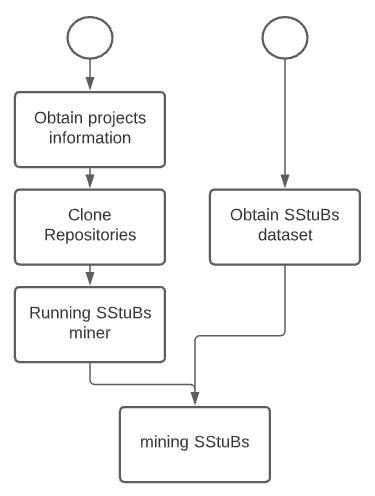
\includegraphics[width=0.7\columnwidth]{figures/process.png}
  \caption{an overview of process}
  \label{fig:process}
\end{figure}


Those 6 communities have quite numbers of projects so we need to harvest the url for each project in order to clone the repository. We use HTTP GET requests to retrieve community pages, which contain a list of projects. Then we use the Jsoup\footnote{\url{https://jsoup.org} [accessed on 12,May 2021]}: a HTML parser to retrieved HTML DOM that contains project urls. At this stage, we remove some projects that have been included the original SStuBs dataset to avoid duplications. All projects are cloned to local disk via a git clone command.
The script that is then used to obtain single statement bugs from each cloned repository is provided by the SStuBs study\footnote{\url{https://github.com/mast-group/mineSStuBs} [accessed on 12,May 2021]}.  Once we have both datasets (original SStuBs and additional datasets from selected software communities), we use a script to identify single statement bugs that are relate to dynamic features. To be precise to what we refer to as dynamic language features, we select keywords from call sites to locate changes in fix commits. Those keywords are provided in Table \ref{tab:keyword}. We select those key words based on Sui et al. \cite{sui2018soundness} - a micro benchmark which contains a collection of usages for dynamic language features.

\begin{table}[h]
\scriptsize
\caption{keywords}
\label{tab:keyword}
\footnotesize
\begin{tabular}{|l|p{5.15cm}|}
\hline
Keyword                  & Full Name                    \\ \hline
.invoke(                 & java.lang.reflect.Method.invoke \\ \hline
.getDeclaredMethod(      & java.lang.Class.getDeclaredMethod\\ \hline
.getDeclaredConstructor( & java.lang.Class.getDeclaredConstructor\\ \hline
.getDeclaredField(       & java.lang.Class.getDeclaredField \\ \hline
.newInstance(            & \multicolumn{1}{l|}{\begin{tabular}[c]{@{}l@{}}java.lang.Class.newIstance\\java.lang.reflect.Constructor.newInstance\end{tabular}}\\ \hline
.forName(                & java.lang.Class.forName         \\ \hline
.findClass(              & java.lang.ClassLoader.findClass  \\ \hline
.defineClass(            & java.lang.ClassLoader.defineClass \\ \hline
.loadClass(              & java.lang.ClassLoader.loadClass   \\ \hline
.readObject(             & java.io.ObjectInputStream.readObject \\ \hline
.allocateInstance(       & sun.misc.Unsafe.allocateInstance     \\ \hline
.getInvocationHandler(   & java.lang.reflect.Proxy.getInvocationHandler\\ \hline
.newProxyInstance(       & java.lang.reflect.Proxy.newProxyInstance    \\ \hline
.load(                   & java.util.ServiceLoader.load           \\ \hline
\end{tabular}
\end{table}

\section{Results and Discussion}
Addition to SStuBs dataset, we mined other 1,032 Java projects from Github. From those projects, we extracted a total of 33,137 single statement bugs.\footnote{SStuBs \cite{karampatsis2020often} has 1,000 projects with 63,923 single statement bugs.} After filtering by keywords provided in Table \ref{tab:keyword}, we found 120 dynamic feature related bugs in SStuBs and 77 in the additional dataset. We then conducted a manual validation to check duplicates and false positives. We ended up with 58 identical single statement bugs. Table \ref{tab:results-overview} shows an overview of a number of bugs for each category.\footnote{Note that there are 4 bugs that appear across multiple categories. The total number of bugs identified is 62.}

\begin{table}[h]
\caption{results overview}
\scriptsize
\label{tab:results-overview}
\footnotesize
\begin{tabular}{|l|l|r|}
\hline
Call site                     &Category& \multicolumn{1}{l|}{\begin{tabular}[c]{@{}l@{}}No. bugs\end{tabular}} \\ \hline
Class.forName                &reflection& 16                                                                             \\ \hline
Method.invoke                &reflection& 15                                                                             \\ \hline
Class.get....                &reflection& 13                                                                             \\ \hline
newInstance                  &reflection& 7                                                                              \\ \hline
classloader                  &dynamic class loading& 5                                                                              \\ \hline
Service.load                 &service loader& 3                                                                              \\ \hline
readObject                   &serialisation& 2                                                                              \\ \hline
Proxy.getInvocationHandler() &dynamic proxy& 1                                                                              \\ \hline
\end{tabular}
\end{table}


32 out of 58 bugs are indicated in the issue tracking system. They provide rich text about why the bug occurs and how to solve it. Furthermore, we analysed the person who reported the issue. Two categories has been identified: (1) community users who encountered issues and therefore reported them. (2) contributor who built the project and identified issues. There are 11/32 issues have been reported by community users and 18/32 have been reported by contributors. We believe that the reported issues by community users provide more piratical scenario that is unlikely to be tested by developers.
%we then disscus it in the conclusion: run test cases to see wether it can be covered or not.
Table \ref{tab:results-fixmethod} shows a number of fix methods for bugs. Those methods have already been discussed in SStuBs \cite{karampatsis2020often}. Most of bugs have been resolved via either providing more arguments for overloaded methods (OVERLOAD\_METHOD\_MORE\_ARGS) or changing arguments (CHANGE\_IDENTIFIER). This indicates dynamic features are likely to be wrongly handled when passing arguments. We discuss some of bugs in more details next.

\begin{table}[h]
\scriptsize
\caption{fix type}
\footnotesize
\label{tab:results-fixmethod}
\begin{tabular}{|l|r|}
\hline
Fix Method                           & \multicolumn{1}{l|}{No. bugs} \\ \hline
OVERLOAD\_METHOD\_MORE\_ARGS       & 26                          \\ \hline
CHANGE\_IDENTIFIER                 & 14                          \\ \hline
SWAP\_BOOLEAN\_LITERAL             & 2                           \\ \hline
LESS\_SPECIFIC\_IF                 & 1                           \\ \hline
OVERLOAD\_METHOD\_DELETED\_ARGS    & 4                           \\ \hline
CHANGE\_CALLER\_IN\_FUNCTION\_CALL & 7                           \\ \hline
DIFFERENT\_METHOD\_SAME\_ARGS      & 5                           \\ \hline
\end{tabular}
\end{table}


\subsection{junit4}
Junit4\footnote{\url{https://junit.org/junit4/} [accessed on 4,June 2021]} is a testing framework, and widely used for Java unit testing. The bug was reported by one of the contributor of the Junit4 repository on Github. The issue describes an ExceptionInInitializerError has been thrown when filtering tests by category, indicating there is an issue with class initialisation. The solution is to add more arguments to \texttt{Class.forName()} method. The class \texttt{java.lang.Class} \cite{javaclassapi} provides two overloading methods to load a class: one with providing the fully qualified name for a class (i.e. \texttt{Class.name("name")}) and another one provides a detailed class loading scenario (i.e. \texttt{Class.name("name", false, getClassLoader())}) by specifying on which class loader that the class will be loaded, and whether this class should be initialised or not.
%should I mention that Class.name("name") is equavenlet to full initialization : Class.name("name", true, getClassLoader())
In this case, a full initialization of a class is not required therefore the second argument should be flagged as false.
%This is a small fix but could be hard for any static analyser/bug detection tool to pick it up as the bug happens at the runtime.


\begin{table}[h!]
  \footnotesize
  \label{tab:junit4}
  \begin{tabular}{rp{5cm}}
    before fix:  &  \footnotesize{\texttt{Class.forName(name);}}\\
    after fix:  &  \footnotesize{\texttt{Class.forName(name, false, getClass().getClassLoader());}} \\
    bug type:   &  \texttt{OVERLOAD\_METHOD\_MORE\_ARGS} \\
    fix commit: &  \texttt{b1068dc55c95d1000e07b71d3a9d9a2fd26bfff9} \\
    commit message:   &  \texttt{Fix for \#359}\\
    issue link &  \url{https://github.com/junit-team/junit4/issues/359}
  \end{tabular}
\end{table}


\subsection{spring-framework}

Spring framework\footnote{\url{https://spring.io/} [accessed on 4,June 2021]} is well-known application framework for Java. A bug was reported on a class \texttt{org.springframework.\\jms.connection.CachedMessageProducer}. It is a model to manage cached message where a reflection is involved. The fix is simple -- an argument has been changed from \texttt{target} to \texttt{CachedMessageProducer.this}. This indicates the target instance that the method is invoked upon has been changed.
%Interestingly insight is that the "target" instance is the super class of CachedMessageProducer. but what is the implication of this? I guess the class requires the specific type of this class.
\begin{table}[h!]
  \footnotesize
  \label{tab:spring}
  \begin{tabular}{rp{5cm}}
    before fix:  &  \footnotesize{\texttt{method.invoke(target, args);}} \\
    after fix:  &  \footnotesize{\texttt{method.invoke(CachedMessageProducer.this, args)}} \\
    bug type:   &  \texttt{CHANGE\_IDENTIFIER} \\
    fix commit: &  \texttt{134e5a2aecf913bcc184d5d3ae845a13d5369078} \\
    commit message:   &  \texttt{Jms2MessageProducerInvocationHandler properly delegates to CachedMess…Issue: SPR-11949}\\
    issue link &  \url{https://github.com/spring-projects/spring-framework/issues/16566}
  \end{tabular}
\end{table}
%spring-projects/spring-framework  Method.invoke()  CHANGE_IDENTIFIER  Jms2MessageProducerInvocationHandler properly delegates to CachedMess…  Collaborator  type: bug https://github.com/spring-projects/spring-framework/issues/16566  https://github.com/spring-projects/spring-framework/commit/134e5a2aecf913bcc184d5d3ae845a13d5369078
\subsection{intellij-community}
Intellij IDEA\footnote{\url{https://www.jetbrains.com/idea/} [accessed on 4,June 2021]} is widely used IDE for many developers. This bug was found at a particular commit that indicated by the commit message: ``A fix for Groovy formatter tests....''.  We also found other 5 bugs that are similar to this pattern, where the call site has been changed with arguments remain the same. The method \texttt{getDeclaredField} \cite{javaclassapi} returns all declared field within the class, whereas the method \texttt{getField} \cite{javaclassapi} returns public member fields of the class. Even though there is no related issue created for it, we believe the fix implies they intend to access public fields via reflection.
\begin{table}[h!]
  \footnotesize
  \label{tab:intellij}
  \begin{tabular}{rp{5cm}}
    before fix:  &  \footnotesize{\texttt{CodeStyleSettings.class.getDeclaredField(name);}} \\
    after fix:  &  \footnotesize{\texttt{CodeStyleSettings.class.getField(name);}} \\
    bug type:   &  \texttt{DIFFERENT\_METHOD\_SAME\_ARGS} \\
    fix commit: &  \texttt{3943eb1f3833c96392538fe671c05d7718a81039} \\
    commit message:   &  \texttt{A fix for Groovy formatter tests (using getField() instead of getDecl…aredField() from CodeStyleSettings).}\\
    issue link &  \url{none}
  \end{tabular}
\end{table}

\section{Conclusion}

In this paper, we have discovered how dynamic language features relate to real-word bugs, especially with single statement bugs. We are surprised that only 58 bugs are found across 2,032 projects. However, given the complicity of analysing dynamic features, we strongly believe those findings can help the program analysis community to improve their tool to detect those bugs.  We want to point out the fact that those bugs are fixed within a single statement -- this implies the cost of fixing such bug is low, and therefore detecting it can be easy as well. From the static analysis point of view, the interests in finding gaps exist in static analysis w.r.t using dynamic language features in Java \cite{sui2020recall} have merged in recent years.  Those mined bugs provide practical sense of how dynamic features are used in real-word projects.

We foresee a number of possible works from this paper.  Since the fix happened within a single statement, we would like to know the scope of the fix candidate, for instance, is the changed identifier in the same method or the same class? This will provide us a good understanding on how close the correct fix to problematic statement, and therefore narrow the analysis scope.

We have discussed the role of bug reporters -- A community user who encountered a bug may have a specific executing scenario. A further analysis of such reported issues, hopefully with full reported stack traces, can help with a better understanding on why it is a bug. Moreover, reported stack traces can be used to feed to static analysis tools \cite{sui2017use} to detect such bug. As project contributors did create issues for those bugs, we are wondering whether the corresponding test can cover it or not. There are two meaning of the word ``cover'': (1) test coverage, such as branch coverage, line coverage. (2) desired program behaviours are tested.

%maybe this is too far away from this study, but it is what I have in my mind.
We found there is a lack of study on the behaviour of dynamic language features, particularly how they being used in real-world programs. A further study on the role of dynamic language features may be required. We would like to know that whether they likely to be used within a program model or act as a bridge that open for other program models. The reason for this concern is the static analysis is usually constrained by analysis scope -- if we want to perform a whole-program analysis then all program models must be included. This is a very issue for a program (as a provider) that is design to open to other program models (i.e. consumer), Spring framework is a good example being a provider that many applications depend on.
% more further works? need to disscus it

% \section{Acknowledgments}



%%
%% The acknowledgments section is defined using the "acks" environment
%% (and NOT an unnumbered section). This ensures the proper
%% identification of the section in the article metadata, and the
%% consistent spelling of the heading.
% \begin{acks}
% To Robert, for the bagels and explaining CMYK and color spaces.
% \end{acks}

%%
%% The next two lines define the bibliography style to be used, and
%% the bibliography file.
\bibliographystyle{ACM-Reference-Format}
\bibliography{ref}

%%
%% If your work has an appendix, this is the place to put it.


\end{document}
\endinput
%%
%% End of file `sample-acmsmall-submission.tex'.
